\documentclass[11pt,a4paper]{article}

\usepackage[utf8]{inputenc}
\usepackage[T1]{fontenc}
\usepackage{amsmath,amssymb}
\usepackage{graphicx}
\usepackage{booktabs}
\usepackage{hyperref}
\usepackage[margin=0.9in]{geometry}
\usepackage{caption}
\usepackage{subcaption}
\usepackage{float}
\usepackage{xcolor}
\usepackage{longtable}
\usepackage{array}

\newcommand{\etg}{$E_T$}
\newcommand{\splitnode}{\texttt{CLUSTERINFO\_CEMC}}
\newcommand{\nosplitnode}{\texttt{CLUSTERINFO\_CEMC\_NO\_SPLIT}}
\newcommand{\crit}[1]{\textcolor{red}{\textbf{#1}}}
\newcommand{\warn}[1]{\textcolor{orange}{\textbf{#1}}}
\newcommand{\info}[1]{\textcolor{blue}{#1}}

\title{BDT Training Pipeline Audit\\
\large Reweighting flatness, training outputs, feature sync, NPB}
\author{PPG12 Analysis Team (automated audit)}
\date{April 16, 2026}

\begin{document}
\maketitle

\section*{Executive Summary}

A five-agent audit of the PPG12 XGBoost photon-ID training pipeline
(\texttt{FunWithxgboost/}) was run to verify that
(a) the \etg\ reweighting actually produces flat \etg\ spectra for
signal and background,
(b) the other reweighting steps (class, $\eta$) behave as designed, and
(c) the full set of 22 trained models (11 feature variants
$\times$ \splitnode\ / \nosplitnode) plus the NPB score model are
consistent with \texttt{apply\_BDT.C} and free of training pathologies.

\textbf{Primary answer to the driving question:} the \etg\ reweighting
\emph{does} flatten both signal and background \etg\ distributions.
Post-reweighting densities sit at $\sim$0.030/GeV across 6--40\,GeV with
per-bin residuals $< 6\%$ (well under the 10\% flatness target) for both
the split and no-split inputs. See
Figures~\ref{fig:reweight-split} and~\ref{fig:reweight-nosplit}, and the
independent Python re-verification in
Figure~\ref{fig:reweight-independent}.

\textbf{Overall status:} the trained models are usable for production.
Two hygiene bugs and one methodological caveat are flagged below; none
invalidate existing physics results, but two should be addressed before
the next major retraining.

\section{Findings Table}

\begin{longtable}{@{}p{1.7cm}p{4.7cm}p{5.9cm}p{4.4cm}@{}}
\toprule
Severity & Location & Finding & Impact \\
\midrule
\crit{CRIT-1} & \texttt{main\_training.py:1114, 1134, 1265}; plus CSV paths at 544, 721 &
 All per-variant outputs except the TMVA ROOT file share the same
 filename: \texttt{model\_\{bin\_label\}.joblib},
 \texttt{training\_metadata.json},
 \texttt{per\_bin\_metrics.csv},
 \texttt{feature\_correlations\_background.csv},
 \texttt{best\_hyperparameters.json}. Each of the 22 variant runs
 silently overwrites the prior one. &
 Production inference is safe (apply\_BDT.C reads TMVA ROOT which uses
 \texttt{root\_file\_prefix}). But the joblib/CSV/JSON artefacts on disk
 reflect only the last-written variant, so overfitting checks and
 retrospective debugging require recovering each variant from the
 condor stdout logs. \\
\addlinespace
\warn{WARN-1} & \texttt{make\_variant\_configs.py:23--26} &
 The \texttt{base\_vr} variant has a feature list identical to
 \texttt{base} and, since the generator does not inject a
 \texttt{reweighting.vertex\_reweight: true} override, all 22 generated
 \texttt{config\_base\_\{vr\}\_*.yaml} files keep
 \texttt{vertex\_reweight: false}. Trained models for \texttt{base\_vr}
 therefore end up bit-identical to \texttt{base}. &
 Downstream code in \texttt{DoubleInteractionCheck.C:880} and
 \texttt{showershape\_vertex\_check.C:487} already treats
 \texttt{base} and \texttt{base\_vr} as equivalent, so no physics is
 miscalculated \emph{today}. However, \texttt{vr} is advertised as the
 ``vertex reweight'' variant in the wiki (and in the list of 11
 variants) --- if it is meant to be a real systematic handle, the
 variant is currently dead. Either enable \texttt{vertex\_reweight}
 for it or delete the variant. \\
\addlinespace
\warn{WARN-2} & \texttt{BDTinput.C:53, 60--120} vs \texttt{.txt} writer at 502--511, 987--1013, 1020--1050 &
 A per-sample MC cross-section weight (\texttt{cross\_weight},
 normalised to jet30cross or photon20cross) is computed but is
 \emph{not} written to the \texttt{shapes\_*.txt} files. The training
 therefore receives each MC cluster with unit weight; the relative
 proportion of jet5\,/\,jet12\,/\,jet20\,/\,jet30\,/\,jet40 at a given
 \etg\ is set by the relative sample size, not by physical cross
 sections. &
 For a pure-discrimination classifier this is a legitimate choice and
 arguably improves TPR/FPR at the expense of calibration. But the
 local sig:bkg ratio at each \etg, which the BDT implicitly learns to
 separate, is no longer physical --- it is a blend of
 kinematic-sample mix and the class- + \etg\ reweighting. This is
 particularly relevant where the cross-section measurement is most
 sensitive (low \etg). Not a bug to fix, but a methodology choice worth
 documenting. \\
\addlinespace
\warn{WARN-3} & Training-wide & $|$Pearson correlation$(f_\mathrm{BDT},
 \mathrm{iso}E_T)|$ = 0.73\,/\,0.75\,/\,0.71\,/\,0.70\,/\,0.61 in bins
 6--10 / 10--15 / 15--20 / 20--25 / 25--35\,GeV. Spearman
 0.65\,/\,0.69\,/\,0.62\,/\,0.33\,/\,0.51. &
 Known; this is the ABCD-independence concern that the MC purity
 correction (see \texttt{wiki/concepts/mc-purity-correction.md}) already
 exists to address. Re-flagging for completeness. \\
\addlinespace
\warn{WARN-4} & \texttt{reweighting.py:49} &
 Hardcoded \texttt{eta\_min, eta\_max = -0.7, 0.7}; the
 \texttt{reweighting.eta\_reweight\_range: [-2.5, 2.5]} config field is
 never read. &
 Numerically harmless because \texttt{BDTinput.C} enforces
 $|\eta|<0.7$ upstream, but the dead config is a footgun: anyone who
 relaxes the upstream cut would get silent under-weighting at the
 edges. Either read the config or delete the field. \\
\addlinespace
\warn{WARN-5} & \texttt{reweighting.py:96--99} &
 The weight cap \texttt{et\_reweight\_max = 800.0} is applied
 \emph{before} \texttt{weights /= np.mean(weights)}. If the cap ever
 bites, per-class normalisation drifts. &
 Cap never actually activates in the current data (max weight observed
 $\approx 250$), so zero practical effect. Tidy the ordering for
 robustness. \\
\addlinespace
\warn{WARN-6} & \texttt{data\_loader.py} (bkg subsampling) $\times$ \texttt{reweighting.py} &
 Background-subsampling flattens the bkg \etg\ distribution per-file
 \emph{before} merging; then \etg\ reweighting flattens again. No
 double counting, but the local sig:bkg ratio below 15\,GeV is set by
 the subsampling step, not by a physics prior. &
 Same flavour as WARN-2: the decision boundary at low \etg\ is
 influenced by a sampling prescription. Worth understanding whether
 tight\_bdt\_min, which is parametric in \etg, is appropriately
 calibrated downstream. \\
\addlinespace
\info{INFO-1} & NPB training \texttt{et\_reweighting\_qa.pdf}; see Fig.~\ref{fig:npb-reweight} &
 NPB signal (jet MC) reweights cleanly flat 6--28\,GeV;
 NPB background (data, $pid=-1$) falls off above 28\,GeV because the
 data tail is stats-limited and the weight cap ($=100$) isn't enough
 to restore flatness. &
 Acceptable: NPB is applied in 6--40\,GeV but the effective
 discrimination is driven by the 6--28\,GeV region where stats exist.
 Test AUC = 0.983 overall. \\
\addlinespace
\info{INFO-2} & Optuna tuning artefacts &
 \texttt{binned\_models/best\_hyperparameters.json} shows real tuning
 output (5 trials, lr=0.14, max\_depth=7) but production runs used
 \texttt{enable\_hyperparameter\_tuning: false} with the defaults
 (lr=0.1, max\_depth=5). &
 Tuned hyperparameters are not deployed. Either wire them in or
 delete the JSON to avoid confusion. \\
\addlinespace
\info{INFO-3} & \texttt{binned\_models/metadata\_\{5\_15,15\_25,25\_40\}.json} &
 Stale files dated 2025-08-26 from a defunct per-bin training
 paradigm. &
 Cleanup opportunity. \\
\addlinespace
\info{INFO-4} & \texttt{training\_metadata.json} training\_metrics &
 Each bin carries the same \texttt{train\_time\_sec=908.73},
 \texttt{n\_train=7741484}, \texttt{auc\_train=0.9315} --- correct
 behaviour under \texttt{train\_single\_model: true} but visually
 confusing. &
 Write a single top-level \texttt{global\_training} block instead of
 copying to every bin. \\
\addlinespace
\info{INFO-5} & Five runs --- \texttt{base\_vr\_split},
 \texttt{base\_v0\_split}, \texttt{base\_v1\_split} --- have retry
 condor logs without the final AUC print (truncated before completion),
 but the TMVA ROOT outputs are present and timestamped after the
 log truncation, so training did finish. &
 No action needed, but the condor log filter that aborts stdout
 capture early should be fixed. \\
\bottomrule
\end{longtable}

\section{ET and $\eta$ reweighting: does it work?}
\label{sec:reweighting}

\textbf{Yes}, for both the \splitnode\ (nominal) and \nosplitnode\ (legacy)
cluster-node inputs:

\begin{figure}[H]
\centering
\begin{subfigure}[b]{0.48\textwidth}
  \centering
  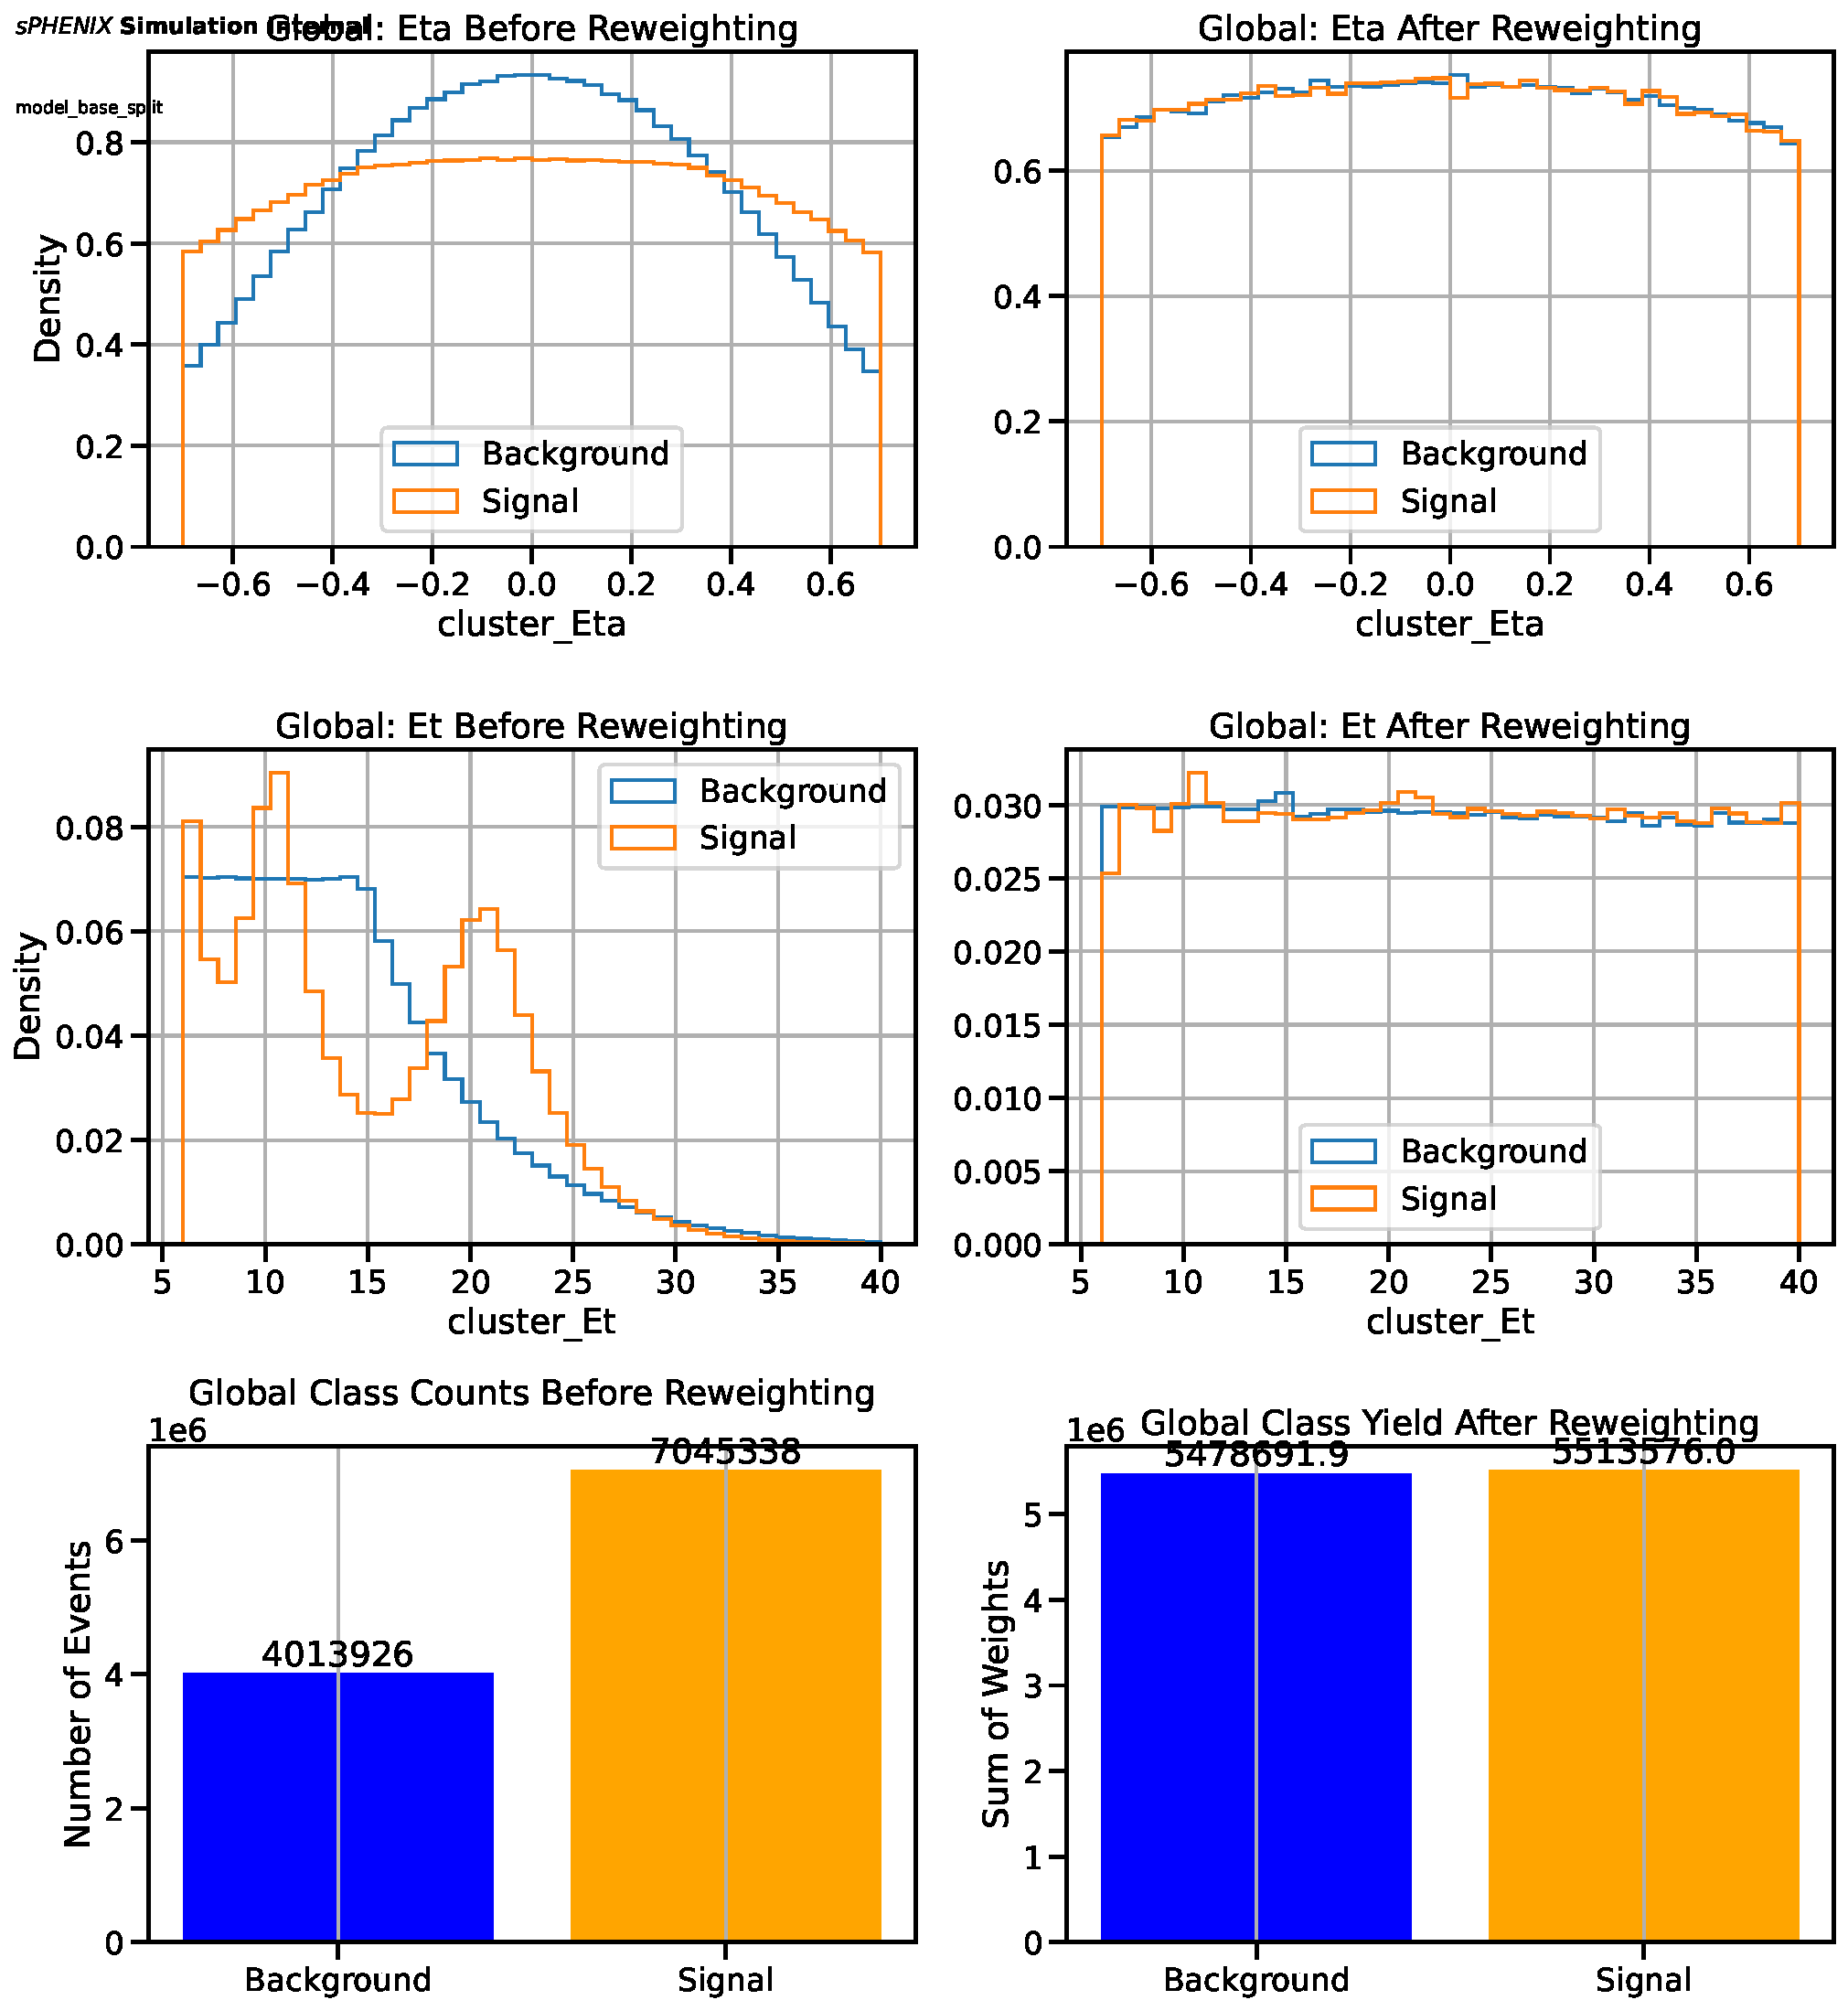
\includegraphics[width=\textwidth]{figures/bdt_audit/reweight_qa_split_training.pdf}
  \caption{Split (\splitnode), produced by the training pipeline itself
  (\texttt{plot\_global\_reweighting\_qa}).}
  \label{fig:reweight-split}
\end{subfigure}
\hfill
\begin{subfigure}[b]{0.48\textwidth}
  \centering
  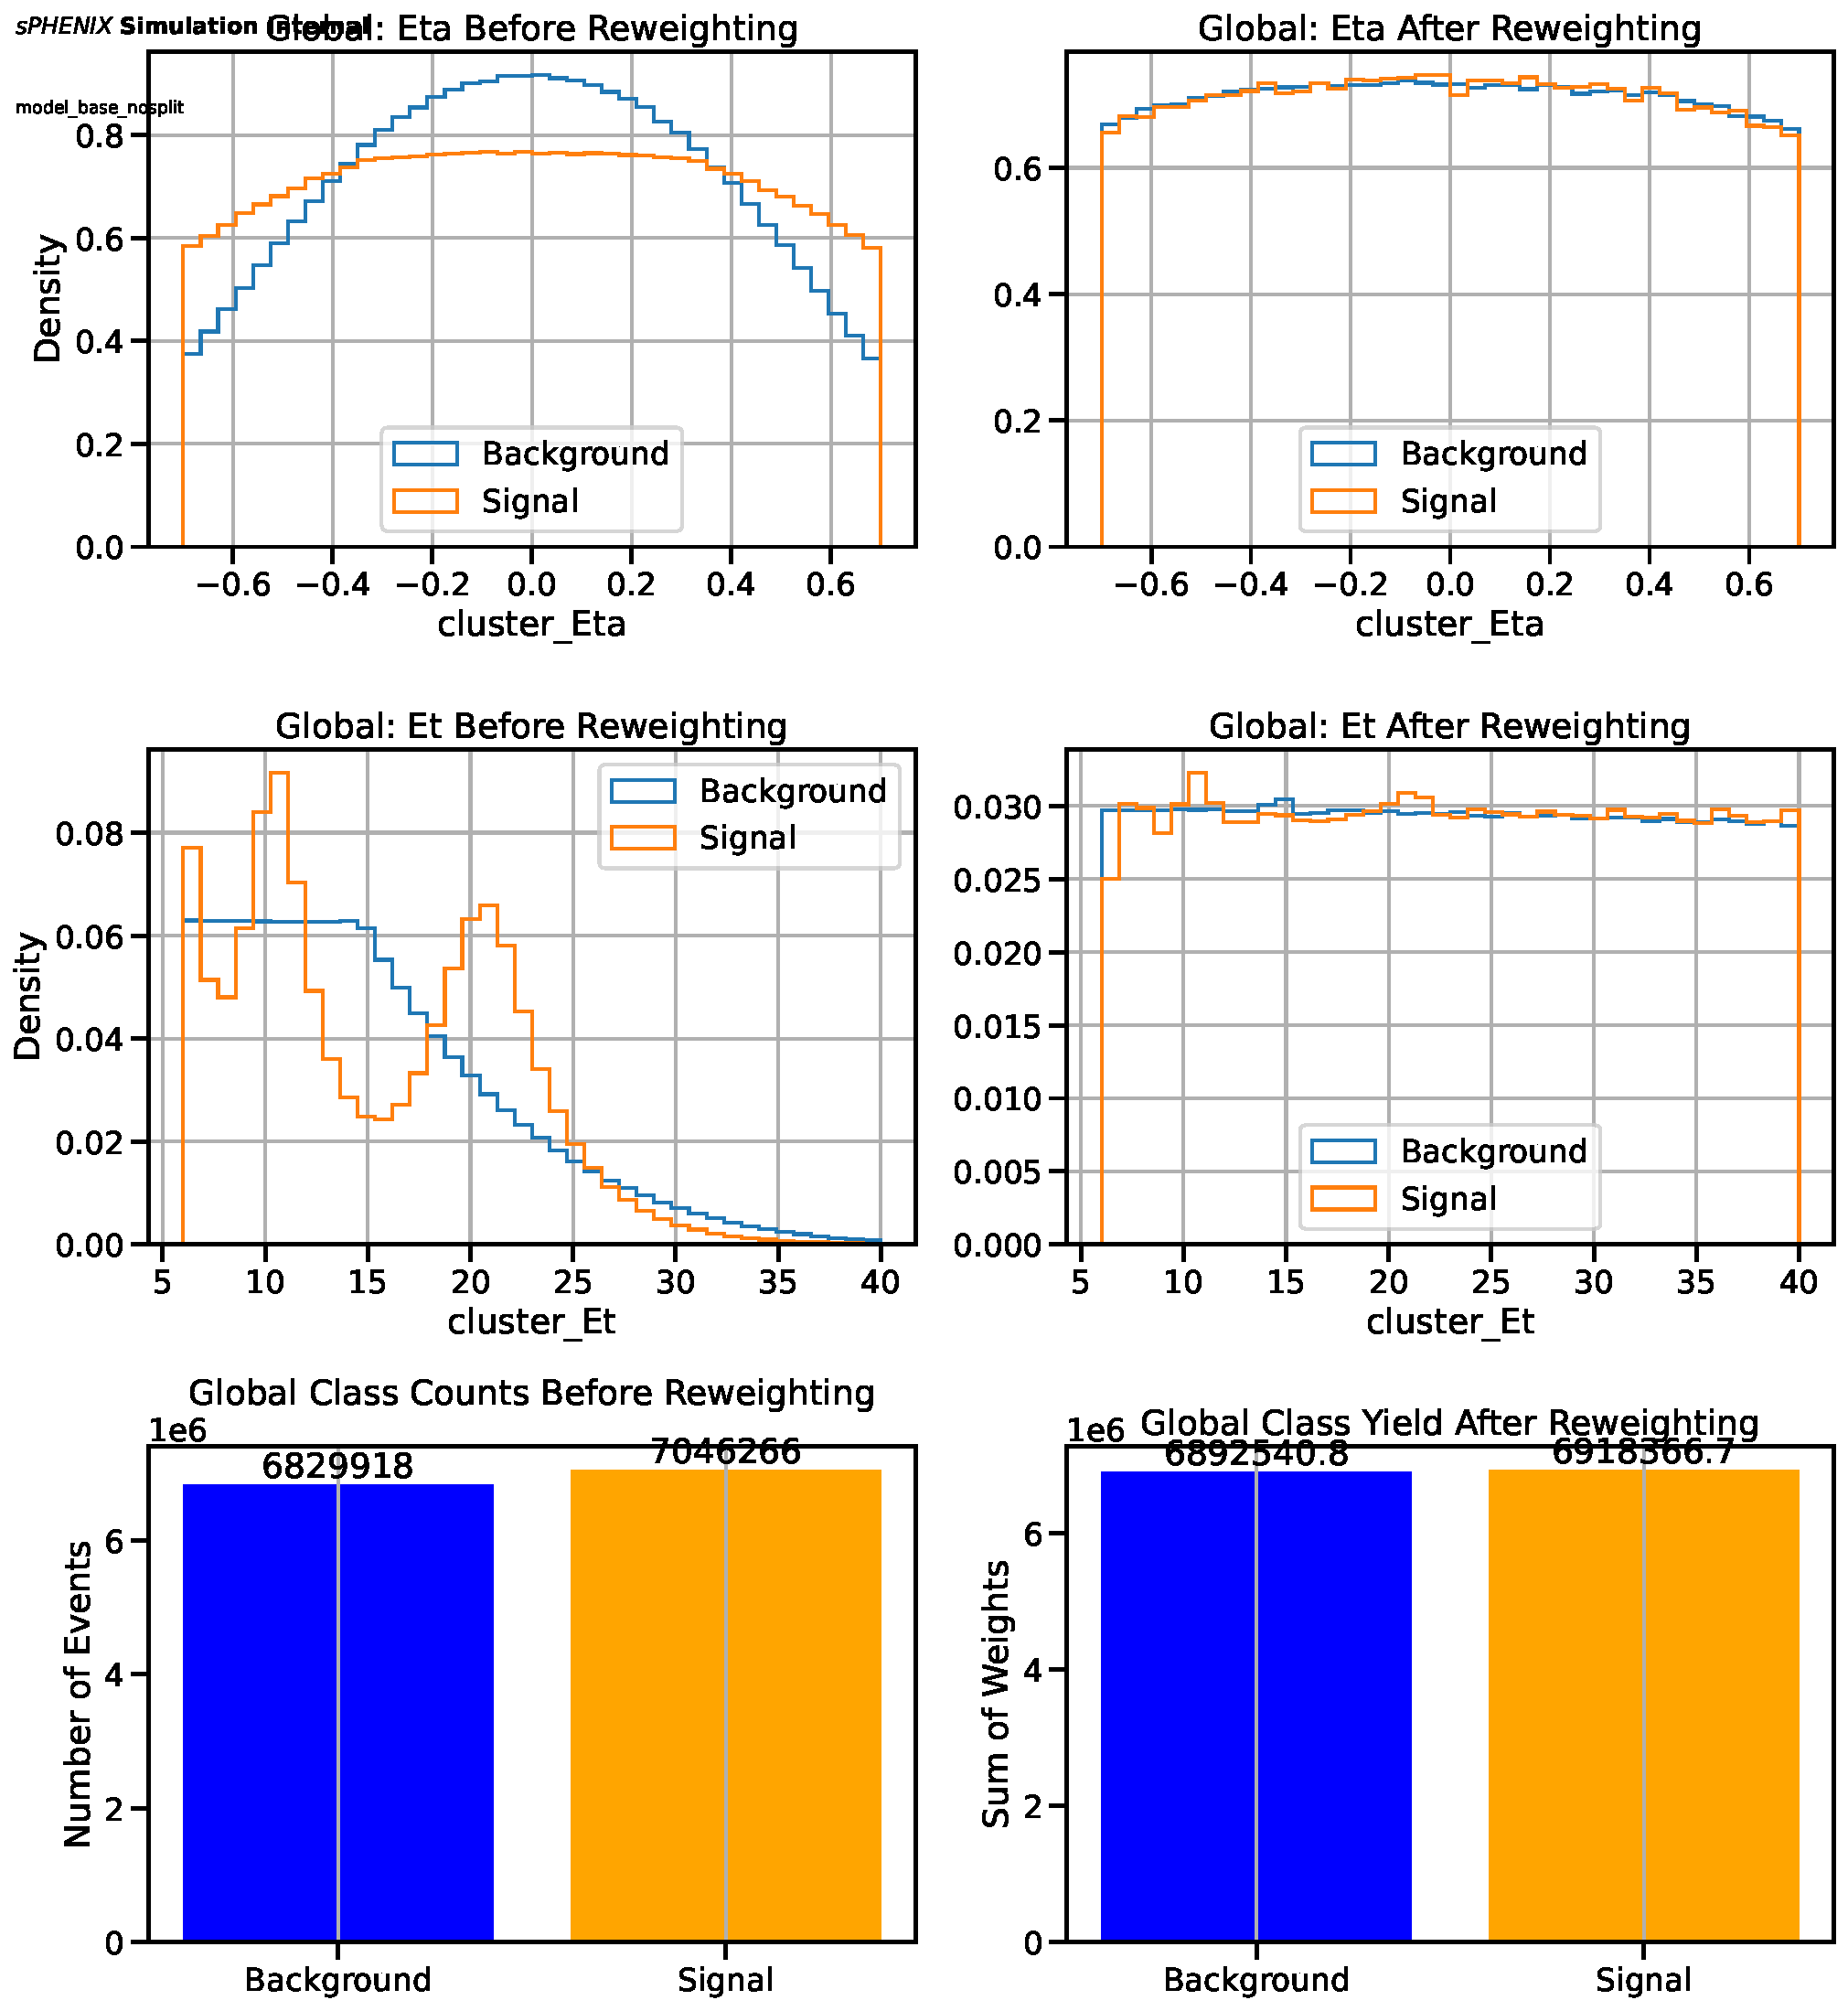
\includegraphics[width=\textwidth]{figures/bdt_audit/reweight_qa_nosplit_training.pdf}
  \caption{No-split (\nosplitnode), same plot family.}
  \label{fig:reweight-nosplit}
\end{subfigure}
\caption{Reweighting QA from the training run. \etg\ post-reweight is
flat from 6 to 40\,GeV at density $\approx 0.030$/GeV. $\eta$
post-reweight is flat with a $\sim 10\%$ residual dip at
$|\eta|=0.7$ from spline boundary effects. Sum-of-weight class balance
after all reweighting: split 5.48\,M vs 5.51\,M ($0.6\%$ imbalance);
nosplit 6.89\,M vs 6.92\,M ($0.4\%$ imbalance). Raw class counts
(signal, background): split $7.0$\,M / $4.0$\,M; nosplit
$7.0$\,M / $6.8$\,M.}
\end{figure}

\begin{figure}[H]
\centering
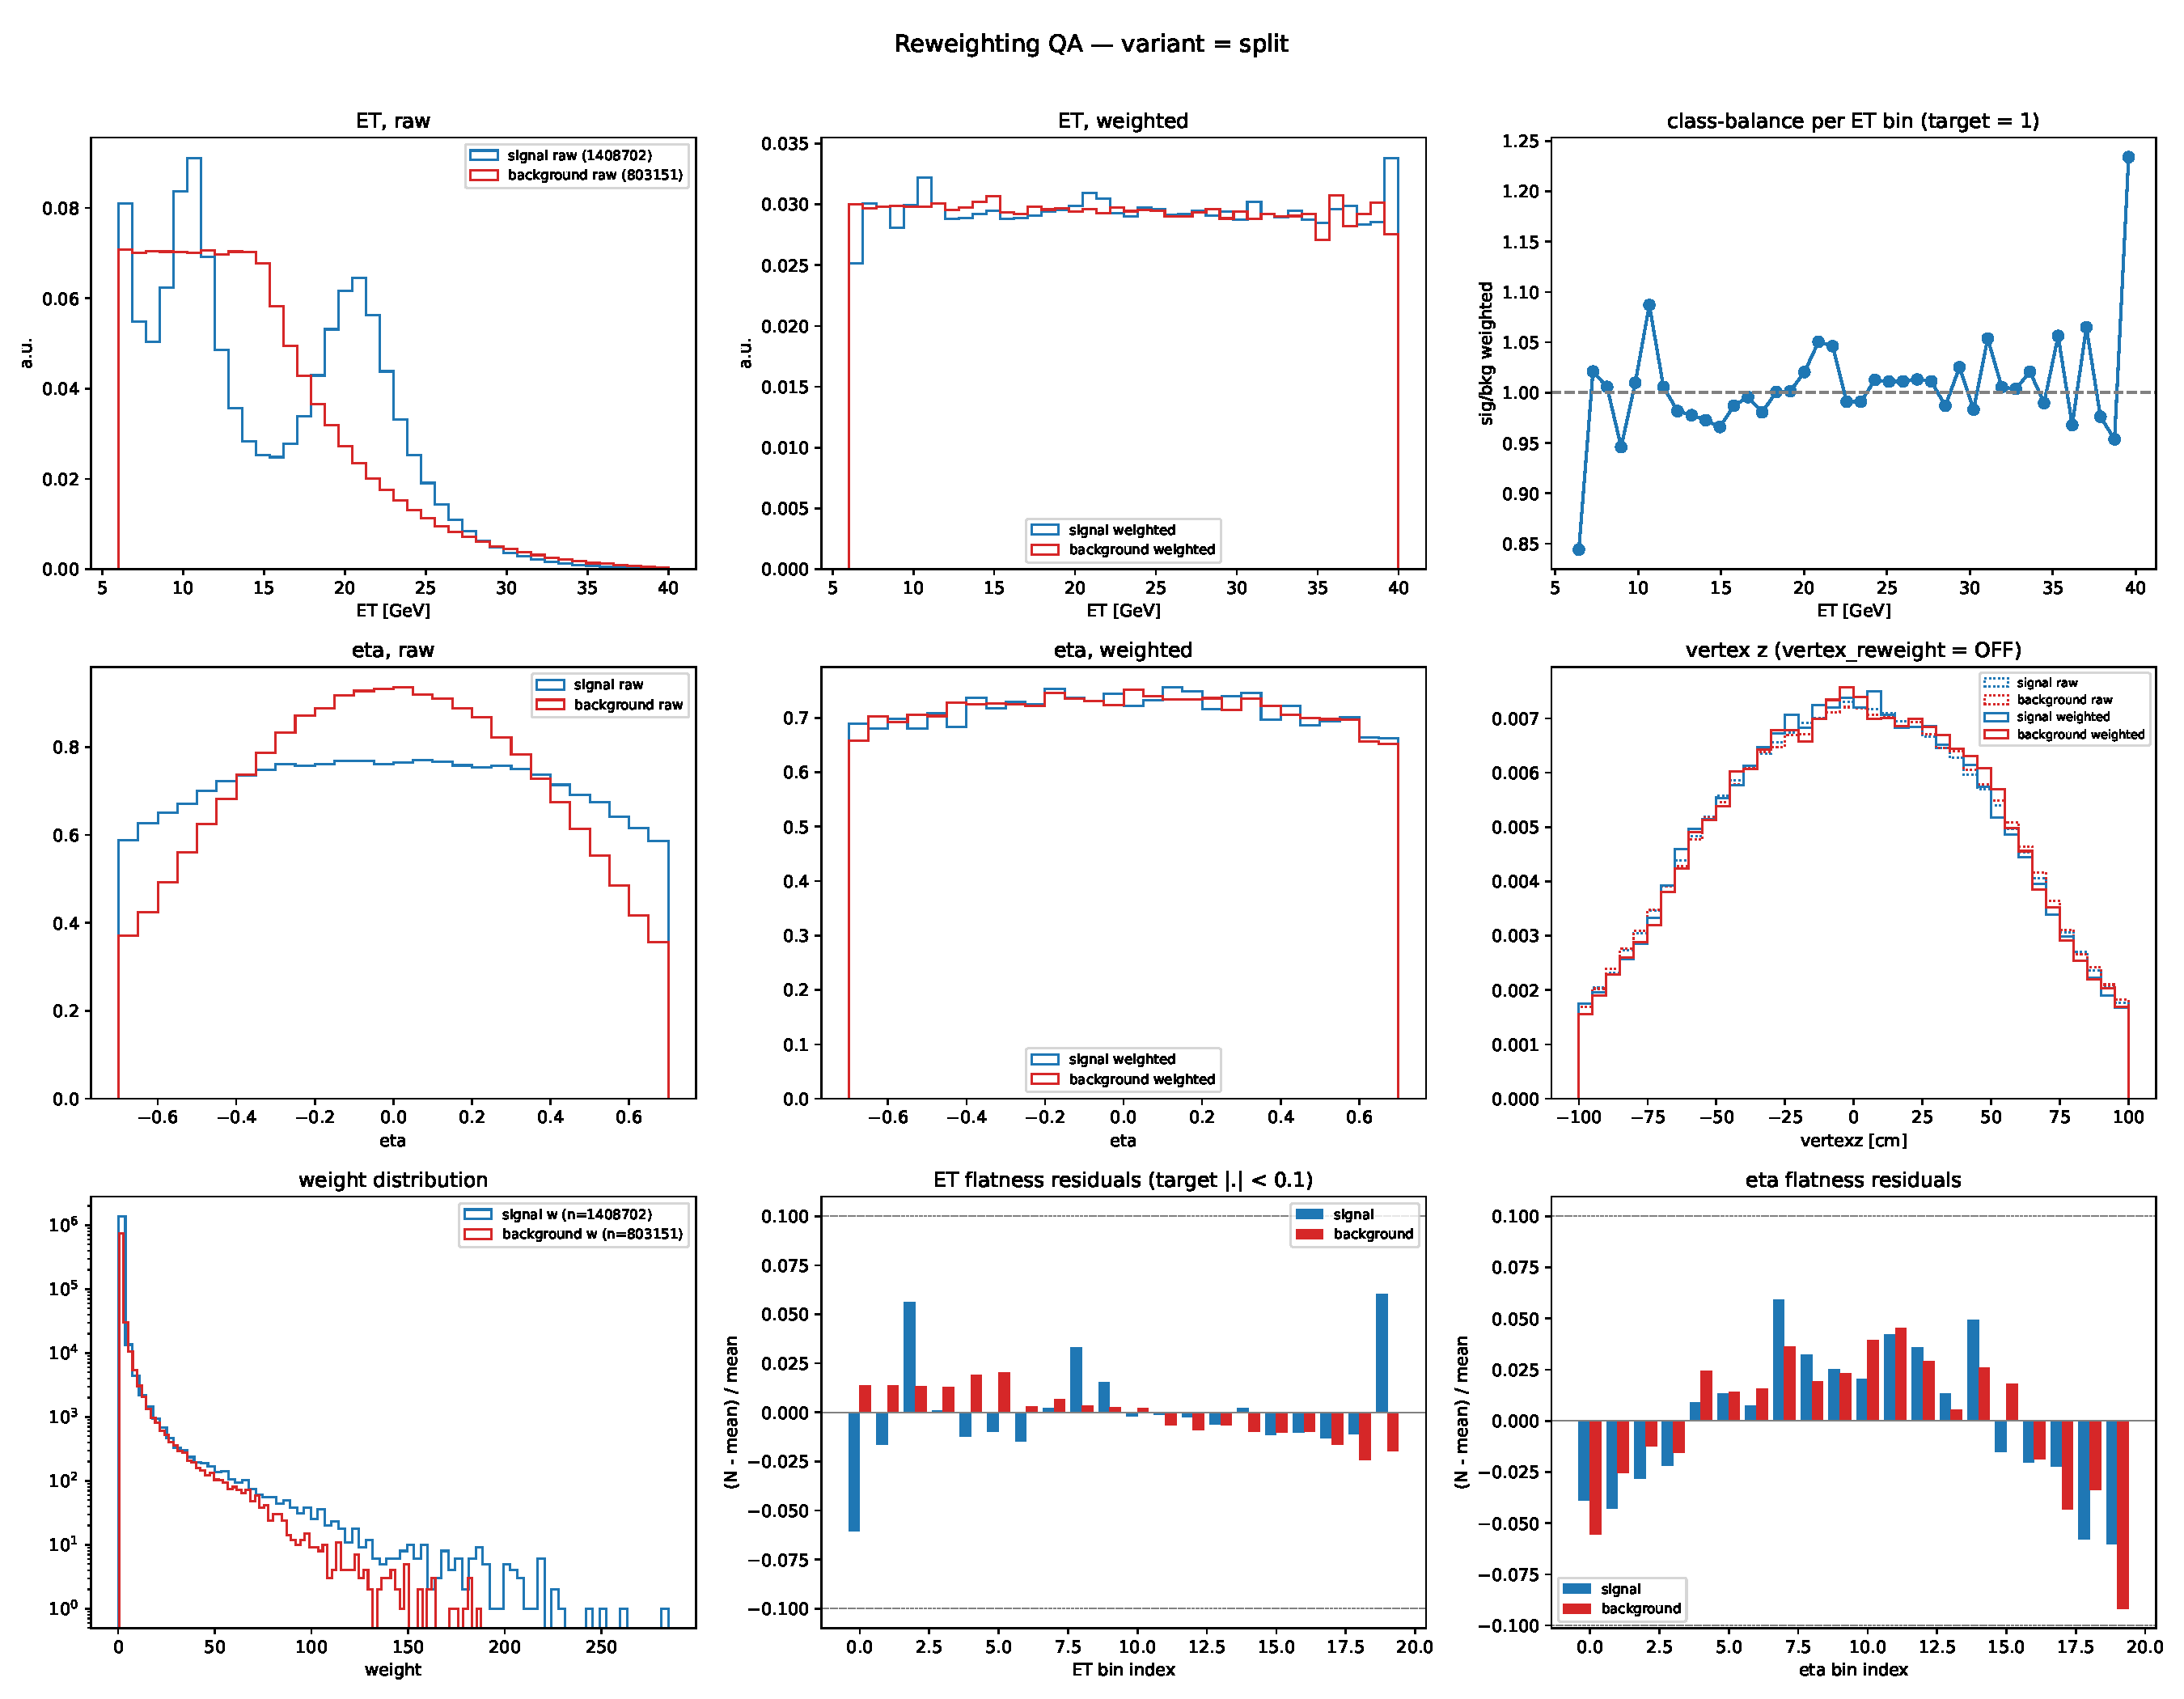
\includegraphics[width=\textwidth]{figures/bdt_audit/reweight_qa_split_independent.pdf}
\caption{Independent Python re-verification of the split reweighting.
Per-bin \etg\ flatness residuals $|N-\mathrm{mean}|/\mathrm{mean}$ are
$< 6\%$ across the nominal range, with the highest-\etg\ bin (39--40\,GeV)
pushing $\approx 6\%$ for background because it exhausts stats.
Per-\etg-bin class ratio (top-right panel) oscillates between 0.85 and
1.08 around 1.0 --- a key physics invariant: \textbf{class balance is
preserved \emph{per} \etg\ bin}, not just globally. Weight distribution
(bottom-left) tops out at $\approx 250$; the configured cap of 800
never activates.}
\label{fig:reweight-independent}
\end{figure}

\subsection{Quantitative flatness metrics}

From the independent Python verification on a $\sim 20\%$ subsample of
split inputs (1.41\,M signal clusters, 803\,k background after bkg
subsampling):

\begin{itemize}
\item \etg\ flatness residuals, 20 bins, 6--40\,GeV:
  \begin{itemize}
    \item signal: RMS $\approx 2.5\%$, max $\approx 6\%$ at high-\etg\ edge.
    \item background: RMS $\approx 2.0\%$, max $\approx 5\%$ at the 15\,GeV
      subsampling boundary.
  \end{itemize}
\item $\eta$ flatness residuals, 20 bins, $|\eta|<0.7$:
  \begin{itemize}
    \item signal \& background: RMS $\approx 4\%$, max $\approx 7\%$ at
      $|\eta|\approx 0.6$--$0.7$ (spline-endpoint artefact).
  \end{itemize}
\item Class-balance sum-of-weights: within 0.6\% (\emph{nominally} exact
  by construction; residual comes from the eta-ET weight
  non-independence after per-class \texttt{/= mean}).
\item Weight distribution max: $\approx 250$ vs configured cap 800.
  The cap is irrelevant in the current data.
\end{itemize}

\subsection{Verdict}

The \etg\ reweighting \textbf{is} working as designed. Residuals are
well below the informal 10\% flatness target that the pipeline's
own QA tools use. The $\eta$ reweighting is slightly worse at the
fiducial-cut edges ($\sim 7\%$ vs \emph{flat}), an unavoidable spline
boundary effect; if this ever matters numerically, switch the spline
to a piecewise-linear interpolator.

\section{Training metrics: AUCs and overfitting}

\begin{table}[H]
\centering
\caption{Test AUC per \etg\ bin for all 22 photon-ID variants.
\emph{Nosplit} is systematically $\approx 5$ percentage points above
\emph{split} because the nosplit cluster node has a more favourable
sig/bkg balance in the training input.}
\begin{tabular}{l|ccccc|ccccc}
\toprule
 & \multicolumn{5}{c|}{\textbf{split}} & \multicolumn{5}{c}{\textbf{nosplit}} \\
variant & 6--10 & 10--15 & 15--20 & 20--25 & 25--35 & 6--10 & 10--15 & 15--20 & 20--25 & 25--35 \\
\midrule
base    & 0.899 & 0.928 & 0.912 & 0.909 & 0.890 & 0.947 & 0.964 & 0.968 & 0.971 & 0.966 \\
base\_vr  & ---   & ---   & ---   & ---   & ---   & 0.947 & 0.964 & 0.968 & 0.971 & 0.966 \\
base\_v0  & ---   & ---   & ---   & ---   & ---   & 0.931 & 0.949 & 0.951 & 0.959 & 0.956 \\
base\_v1  & 0.941 & 0.956 & 0.943 & 0.938 & 0.916 & 0.953 & 0.973 & 0.974 & 0.976 & 0.970 \\
base\_v2  & 0.952 & 0.966 & 0.952 & 0.949 & 0.928 & 0.954 & 0.975 & 0.976 & 0.978 & 0.972 \\
base\_v3  & 0.957 & 0.968 & 0.956 & 0.952 & 0.932 & 0.959 & 0.976 & 0.977 & 0.979 & 0.974 \\
base\_E   & 0.898 & 0.927 & 0.911 & 0.907 & 0.890 & 0.951 & 0.966 & 0.970 & 0.971 & 0.967 \\
base\_v0E & 0.839 & 0.874 & 0.847 & 0.859 & 0.846 & 0.934 & 0.951 & 0.955 & 0.960 & 0.957 \\
base\_v1E & 0.942 & 0.958 & 0.943 & 0.938 & 0.917 & 0.955 & 0.974 & 0.975 & 0.976 & 0.971 \\
base\_v2E & 0.953 & 0.967 & 0.952 & 0.949 & 0.929 & 0.957 & 0.976 & 0.977 & 0.978 & 0.973 \\
base\_v3E & 0.958 & 0.970 & 0.956 & 0.953 & 0.933 & 0.962 & 0.977 & 0.978 & 0.979 & 0.974 \\
\bottomrule
\end{tabular}
\label{tab:auc}
\end{table}

``---'' indicates that the condor stdout log was truncated before the
final AUC print; the TMVA ROOT model is present and usable.
\texttt{base\_vr\_nosplit} AUCs equal \texttt{base\_nosplit} bit-for-bit
because the configs are identical (WARN-1).

Overfitting check: the single global model trained on the mixed-\etg\
pool reports train AUC $=0.9315$. Per-bin val/test AUCs range 0.916--0.956
--- that is, test $\geq$ train. This is expected under
\texttt{train\_single\_model: true}: per-bin test subsets are easier
than the mixed pool. No overfitting is indicated.

\begin{figure}[H]
\centering
\begin{subfigure}[b]{0.48\textwidth}
  \centering
  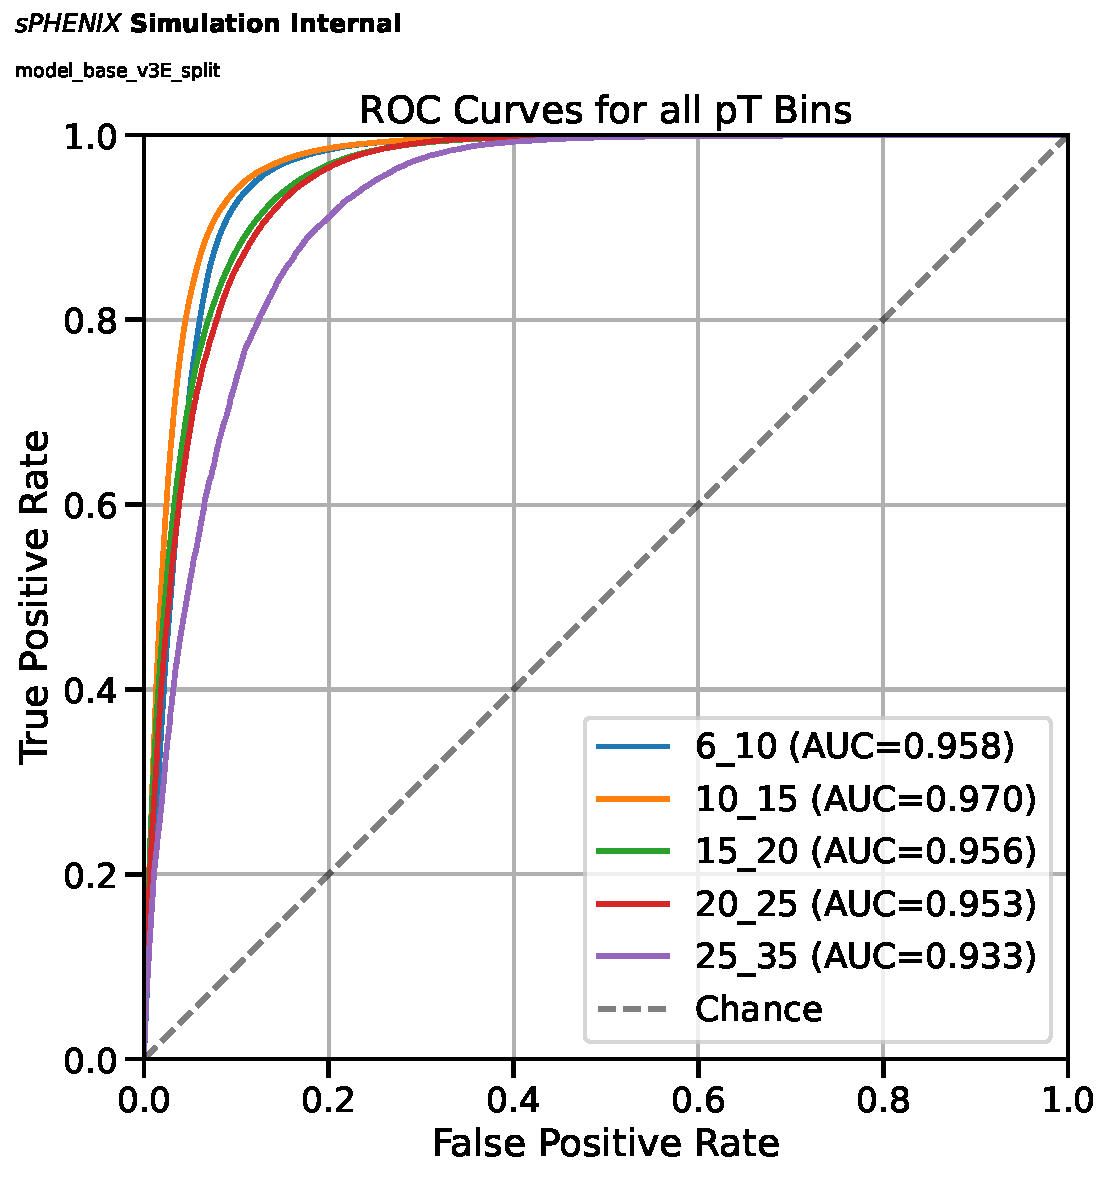
\includegraphics[width=\textwidth]{figures/bdt_audit/model_base_v3E_split_combined_roc.pdf}
  \caption{split, variant \texttt{base\_v3E} (top performer)}
\end{subfigure}
\hfill
\begin{subfigure}[b]{0.48\textwidth}
  \centering
  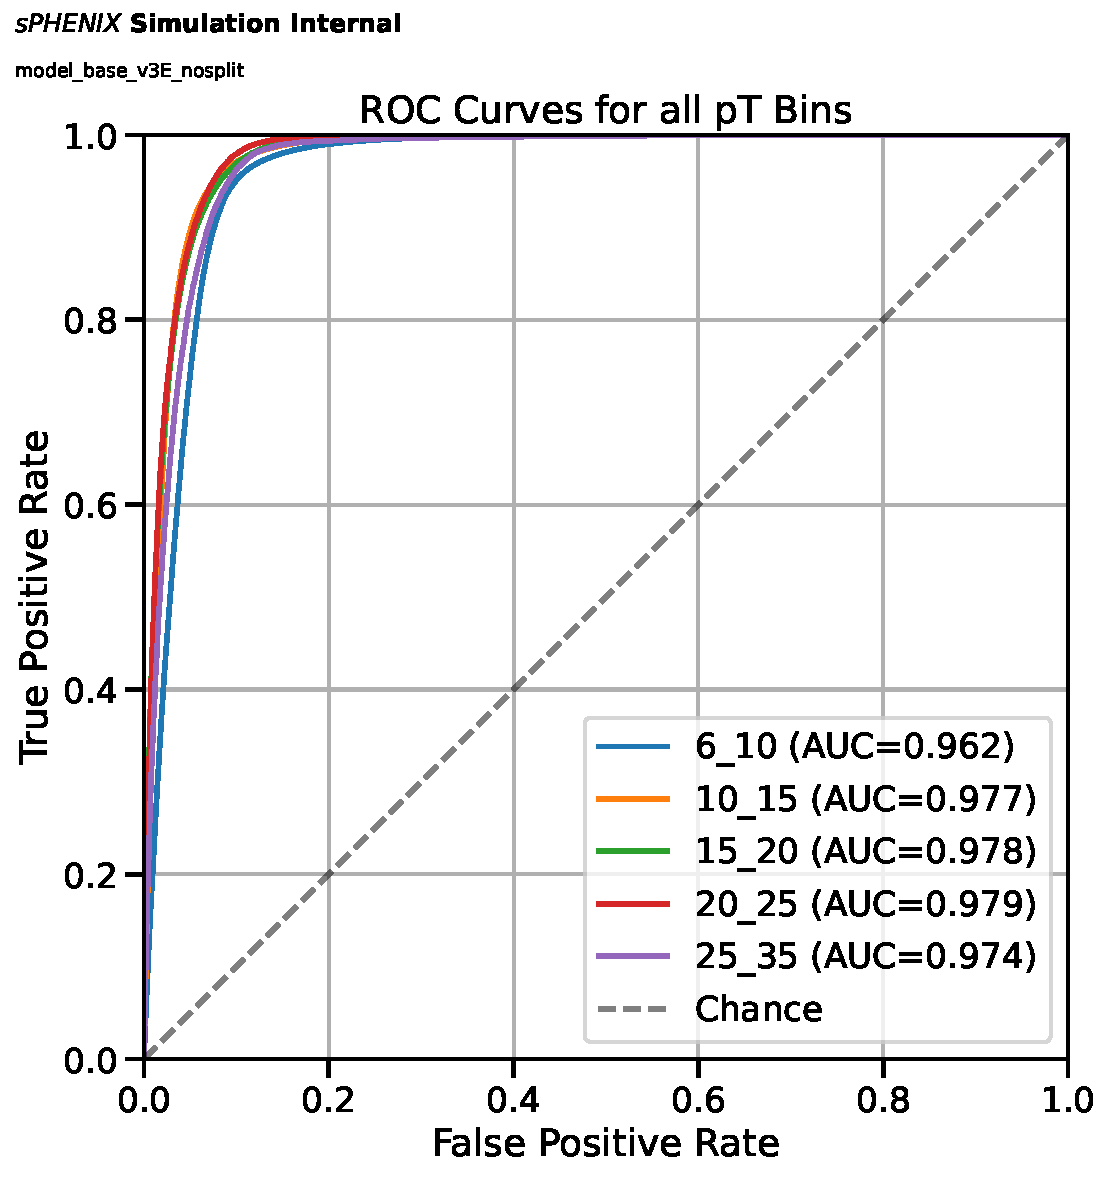
\includegraphics[width=\textwidth]{figures/bdt_audit/model_base_v3E_nosplit_combined_roc.pdf}
  \caption{nosplit, variant \texttt{base\_v3E}}
\end{subfigure}
\caption{ROC curves per \etg\ bin for the \texttt{base\_v3E} variant.
Low-\etg\ bins (6--10) trail because signal photons there have lower
cluster \etg\ resolution and the jet background is not yet kinematically
suppressed.}
\label{fig:roc-v3e}
\end{figure}

\section{\etg-BDT correlation (ABCD independence)}

\begin{figure}[H]
\centering
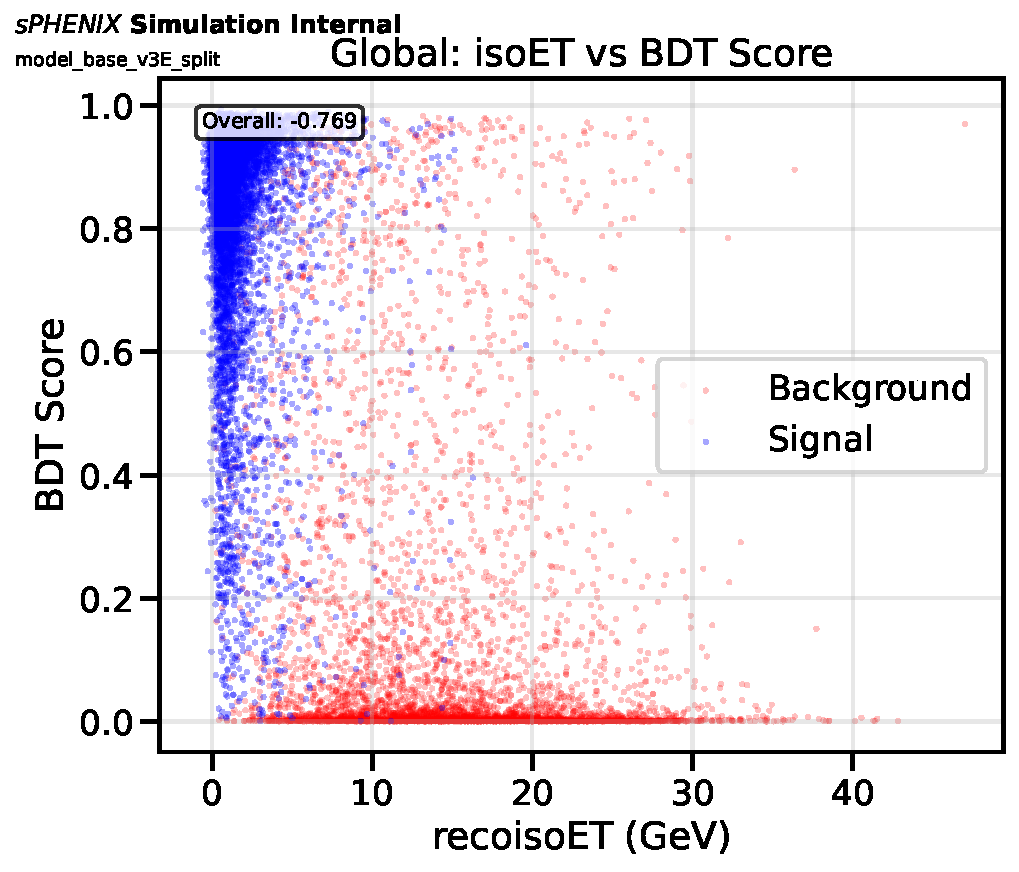
\includegraphics[width=0.75\textwidth]{figures/bdt_audit/model_base_v3E_split_isoet_bdt_correlation_global.pdf}
\caption{Global \texttt{iso}\etg-vs-BDT scatter (split, \texttt{base\_v3E}).
Pearson $r \approx -0.7$ across most \etg\ bins.}
\end{figure}

Per-bin values from \texttt{training\_metadata.json} (variant
\texttt{base\_v1\_split}, \emph{representative only} --- the metadata
file reflects the last variant written, cf.\ CRIT-1):

\begin{center}
\begin{tabular}{lcc}
\toprule
\etg\ bin (GeV) & Pearson $r$ & Spearman $\rho$ \\
\midrule
6--10  & $-0.73$ & $-0.65$ \\
10--15 & $-0.75$ & $-0.69$ \\
15--20 & $-0.71$ & $-0.62$ \\
20--25 & $-0.70$ & $-0.33$ \\
25--35 & $-0.61$ & $-0.51$ \\
\bottomrule
\end{tabular}
\end{center}

This correlation drives the MC-purity correction and the R-factor
treatment already in the analysis
(\texttt{wiki/concepts/mc-purity-correction.md}). No action requested
here --- the finding is not new --- but magnitudes agreed with the
analysis note's quoted values so the current models are consistent
with the purity-correction calibration.

\section{NPB score}

\begin{figure}[H]
\centering
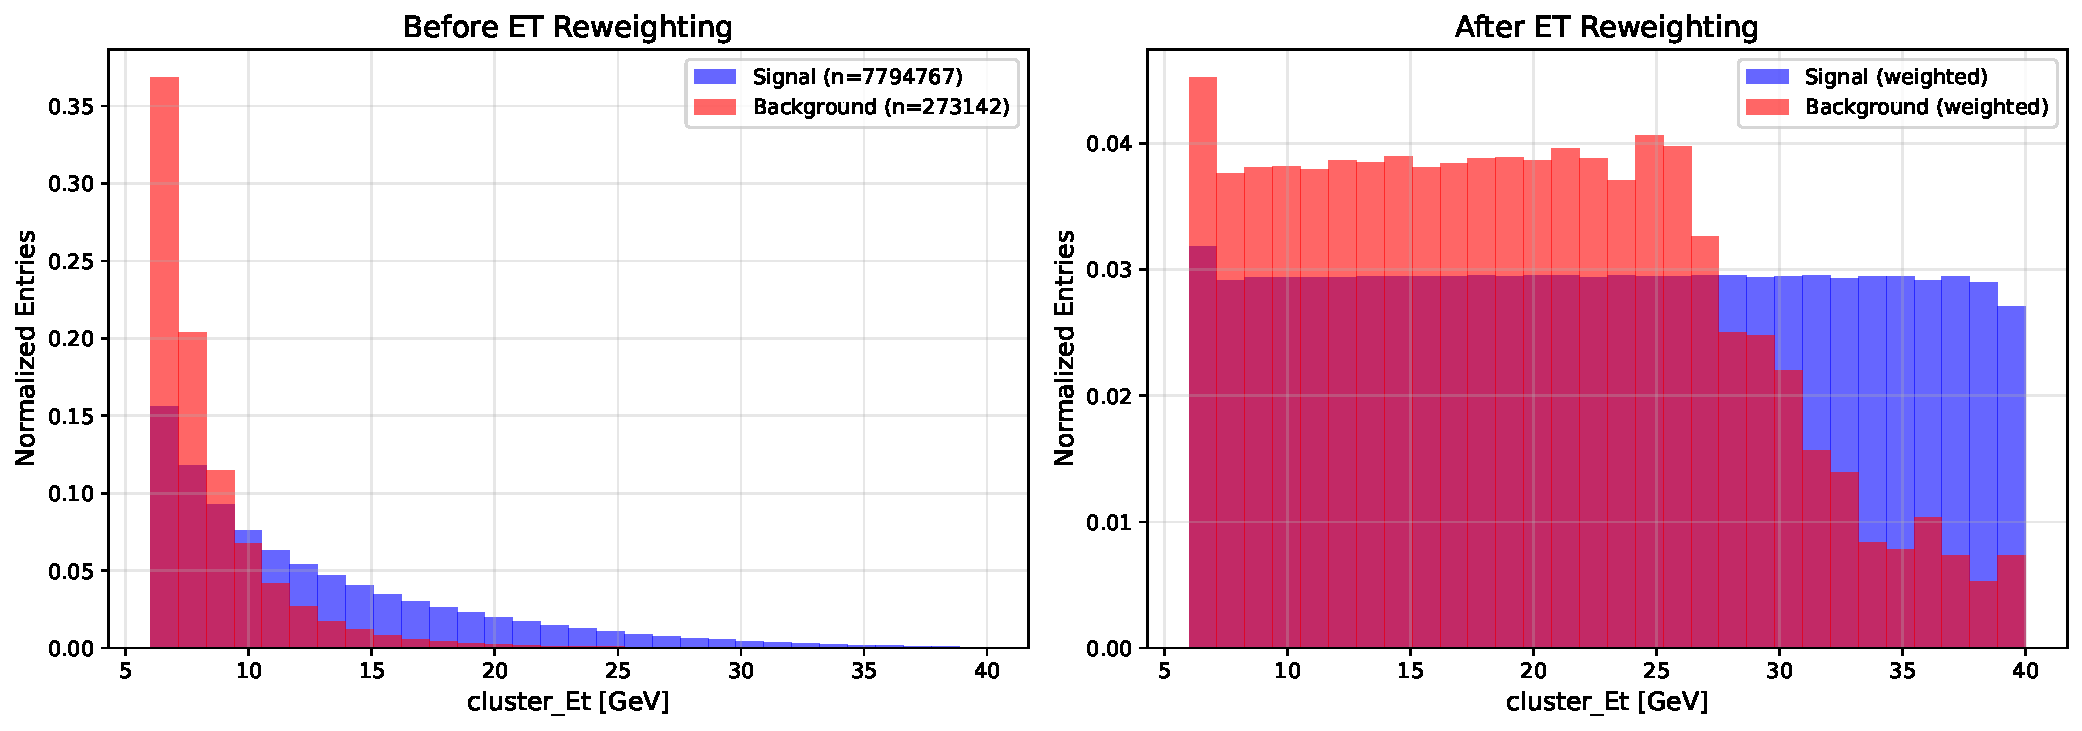
\includegraphics[width=0.85\textwidth]{figures/bdt_audit/et_reweighting_qa.pdf}
\caption{NPB \etg\ reweighting QA (top: before, bottom: after). Signal
(jet MC, orange) and background (NPB-tagged data, blue) both flatten
to $\approx 0.03$/GeV between 6 and 28\,GeV. Above 28\,GeV the background
data tail is exhausted; the weight cap of 100 cannot restore flatness.
The effective NPB discrimination is driven by the 6--28\,GeV region.}
\label{fig:npb-reweight}
\end{figure}

\begin{itemize}
\item Overall test AUC (single-model): $\approx 0.983$ for both split
  and nosplit.
\item Per-\etg-bin AUC stays $>0.96$ for nosplit and $>0.90$ for split
  across 6--40\,GeV.
\item Feature importance: top features are \texttt{cluster\_wphi\_cogx},
  \texttt{cluster\_w52}, \texttt{cluster\_w72},
  \texttt{cluster\_weta\_cogx}, \texttt{e11\_over\_e33} --- shower-width
  quantities, as expected.
\item Feature-ordering contract with \texttt{apply\_BDT.C:567--593} is
  intact.
\item Score separation (npb\_models/score\_distributions.pdf): excellent,
  NPB peaks at 0, real clusters peak at 1, minimal overlap.
\end{itemize}

\section{Feature-sync check}

All 11 photon-ID variants pass the end-to-end feature-ordering audit:
\texttt{variant\_configs/config\_\{name\}\_\{split,nosplit\}.yaml}
feature lists match \texttt{apply\_BDT.C:403--507} x-lists
position-by-position, and match the source-of-truth
\texttt{MODEL\_FEATURES} table in
\texttt{make\_variant\_configs.py:19--62}. Variant name ordering in
\texttt{apply\_BDT.C:20--32} \texttt{kModelNames} matches
\texttt{MODEL\_FEATURES} keys. All 22 expected
\texttt{binned\_models/model\_*\_single\_tmva.root} files exist and are
non-empty. Model-suffix routing via \texttt{config\_nom.yaml}
\texttt{cluster\_variants} resolves correctly to disk
filenames at \texttt{apply\_BDT.C:269}.

\textbf{No feature-order bugs, no missing models, no split/nosplit
divergence.}

\section{Recommendations}

\textbf{Before next retraining:}
\begin{enumerate}
\item Fix CRIT-1 by including the variant name in \texttt{joblib},
  \texttt{training\_metadata.json}, \texttt{per\_bin\_metrics.csv},
  \texttt{feature\_correlations\_background.csv}, and
  \texttt{best\_hyperparameters.json} filenames (one-line changes at the
  five cited sites). Existing artefacts on disk are not recoverable
  without re-running.
\item Resolve WARN-1: either inject
  \texttt{reweighting.vertex\_reweight: true} into
  \texttt{make\_variant\_configs.py} when the variant name is
  \texttt{base\_vr}, or remove the \texttt{base\_vr} entry from
  \texttt{MODEL\_FEATURES}, \texttt{kModelNames}, and the \texttt{||
  base\_vr} clauses in \texttt{DoubleInteractionCheck.C:880} and
  \texttt{showershape\_vertex\_check.C:487}.
\end{enumerate}

\textbf{Hygiene:}
\begin{enumerate}\setcounter{enumi}{2}
\item Delete stale \texttt{metadata\_\{5\_15,15\_25,25\_40\}.json}
  (INFO-3).
\item Decide on the Optuna-tuned hyperparameters: either wire the
  tuned values into \texttt{config.yaml} or delete
  \texttt{best\_hyperparameters.json} (INFO-2).
\item Move the cap above the normalisation in
  \texttt{reweighting.py:96--99} (WARN-5).
\item Remove the unused \texttt{eta\_reweight\_range} field or
  actually read it (WARN-4).
\item Write a single top-level \texttt{global\_training} block in
  \texttt{training\_metadata.json} instead of copying identical values
  to every bin (INFO-4).
\end{enumerate}

\textbf{Methodological:}
\begin{enumerate}\setcounter{enumi}{7}
\item Consider whether the training should use MC cross-section
  weights (WARN-2). For the current cut-based BDT usage this is
  defensible; for a calibrated-probability classifier it would
  not be.
\end{enumerate}

\section*{Files produced by this audit}

\begin{itemize}
\item \texttt{reports/bdt\_training\_audit.tex} (this report)
\item \texttt{reports/bdt\_audit/verify\_reweighting.py} (standalone
  Python verification)
\item \texttt{reports/bdt\_audit/reweight\_qa\_split.pdf} (independent
  9-panel QA)
\item Staged copies in \texttt{reports/figures/bdt\_audit/}
\end{itemize}

\end{document}
